\documentclass[a4paper]{ifacconf}

\makeatletter
\let\old@ssect\@ssect % Store how ifacconf defines \@ssect
\makeatother

\usepackage{graphicx}

\usepackage[numbers]{natbib}
\bibliographystyle{plainnat}

\usepackage{siunitx}
\usepackage{amsmath}

\usepackage[hidelinks]{hyperref}

\makeatletter
\def\@ssect#1#2#3#4#5#6{%
    \NR@gettitle{#6}% Insert key \nameref title grab
    \old@ssect{#1}{#2}{#3}{#4}{#5}{#6}% Restore ifacconf's \@ssect
}
\makeatother

\newcommand{\DT}{\ensuremath{{\Delta}T}}


\begin{document}
    
    \begin{frontmatter}
        \title{Final Project for Service Design and Engineering}
        \author{Daniele Parmeggiani}
        \date{2023-01-05}
    \end{frontmatter}
    
    \section{Introduction}
    
    The developed project named Kappa aims at providing a service capable of letting a user upload and run arbitrary code, through the composition of independent services.
    This is conceptually similar to the AWS Lambda service.\footnote{
        See \url{https://aws.amazon.com/lambda/}.
    }
    
    The submitted composition of services is presented in detail in \S\ref{sec:structure}, while their implementation is outlined in \S\ref{sec:implementation}.
    Section~\ref{sec:workflow} below portrays the experience of a user making use of the service provided.
    
    The implementation has been submitted and is also available at \url{https://github.com/dpdani/sde-project}.
    
    
    \section{The Workflow}\label{sec:workflow}
    
    A user of the Kappa service can perform the following workflow:
    
    \begin{enumerate}
        \item sign up;
        \item log in;
        \item create a function (i.e. upload a function's code);
        \item however many times:
        \begin{enumerate}
            \item execute the function;
            \item check the function's logs;
        \end{enumerate}
        \item check the billing status;
        \item delete the function.\footnote{
            An example run mimicking the above workflow is available at \url{https://github.com/dpdani/sde-project/blob/main/report/example-run.txt}.
        }
    \end{enumerate}

    Notice that the function's code to be executed will need to be Python code: the entire system is implemented entirely in Python and for simplicity the arbitrary code is loaded using Python's own utilities.
    In order to use other languages there would need to be further development.
    
    Overall, six services and one command line client have been developed.
    
    \section{Design of the Services}\label{sec:structure}
    
    Let us go through the design of each service individually and later outline the principles around their composition.
    
    The core service developed is Kappa Runner: it provides the actual runtime in which the user functions will run.
    It is distinctively disjoint from the Kappa Functions Logs and Code services: these are intended to offload the need for Kappa Runner to hold a persistency layer of its own.
    The Kappa Functions Code service holding of the user-input code, also makes it possible to have multiple instances of the Runner service running independently and to restore the runtime of running functions.
    Such is so, because it is possible to fetch a copy of the code from each instance of Kappa Runner at any time; although these behaviors have not been implemented, as detailed in \S\ref{sec:improvements}.
    The Functions Logs service also offloads historical querying of functions behavior from the Runner service, i.e. the Kappa service described below need not query Kappa Runner which is intended to be already loaded with the executions of users functions.
    
    The Kappa Logs service is intended as an abstraction for logs the user may find interesting (which are exposed partly in Kappa Functions Logs and partly in Kappa Data) to be used by the Kappa service.
    
    Kappa Data exposes the storage for user data and functions, which is shared between the different components detailed here.
    
    Lastly, the Kappa service provides a coherent user-facing set of APIs that are intended to orchestrate the various sub-systems described above, providing to the end user an experience consistent with the workflow presented above in \S\ref{sec:workflow}, without them needing to be aware of the underlying complexity of the various sub-systems.
    
    GitHub is used to provide an external data source to show possibly interesting public repositories to the end user, at function creation time.

    The distinctive feature of composing the various services, instead of holding all of their functionalities in one ubiquitous system, makes it possible not only to scale up computing capacity for user functions independently of the rest of the system, but also to decouple and share application logic between the services.
    
    \begin{figure}
        \centering
        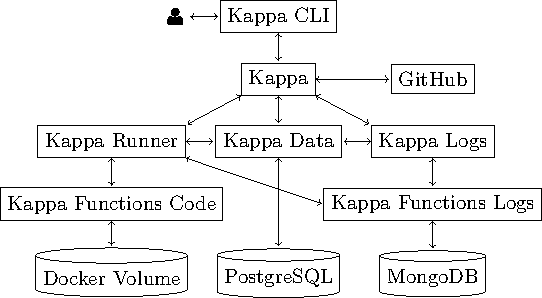
\includegraphics[width=0.9\linewidth]{figures/structure}
        \caption{Structure and interactions of the services.}
        \label{fig:structure}
    \end{figure}

    In Figure~\ref{fig:structure} there is a depiction of the developed services and of their interactions.
    
    \subsection{Logical Layers}
    
    With regards to the four logical layers described in the assignment, the developed services are:
    
    \begin{itemize}
        \item Process layer: 
        \begin{itemize}
            \item orchestration between the services (\texttt{kappa})
        \end{itemize}
        \item Business logic layer:
        \begin{itemize}
            \item function runtime, and billing logic (\texttt{kappa-runner})
        \end{itemize}
        \item Adapter layer:
        \begin{itemize}
            \item unified logs (\texttt{kappa-logs})
        \end{itemize}
        \item Data layer:
        \begin{itemize}
            \item user data and logs emitted by the system (\texttt{kappa-data})
            \item logs emitted by functions (\texttt{kappa-fn-logs})
            \item stored functions code (\texttt{kappa-fn-code})
        \end{itemize}
    \end{itemize}
    
    \subsection{The CLI Client}
    
    It not being a service per se, the CLI client is what is intended to be the interface for the service as a whole, i.e. the intended client for Kappa; notwithstanding the possibility for users to make HTTP calls directly to Kappa.
    Its design is thus not intended to be a crucial part of the overall system, while it is instead intended to provide a pleasing experience to the end user.
    
    \section{Implementation of the Services}\label{sec:implementation}
    
    As already mentioned, the six services, and the CLI client too, have been developed in Python.
    Each of them is stored in a separate folder in the project, and can be run in a Docker container; see \S\ref{sec:docker} below for details on building and running the provided containers.
    
    They all are implemented using a web framework called FastAPI.
    As explained later, this library has been useful not only for exposing the services themselves, but also for creating client libraries that are used in turn by the services to communicate to one another, see \S\ref{sec:openapi} for further details.
    
    There is no implementation of a service discovery as part of this submission, each service holds a configuration file that lists at which host the other services can be found.
    The configuration files also hold access information for connecting to PostgreSQL and MongoDB.
    
    \subsection{Structure of the Submission}
    
    At the root folder of the submission there can be found seven folders comprising the source code of the six developed services and client.
    Each of them essentially follows the same pattern of having a Python package containing the code and a configuration file along with it.
    The \texttt{libs/} folder contains the automatically generated client libraries, see the below \S\ref{sec:openapi} for details.
    
    There can also be found a \texttt{pyproject.toml} file which is used by the Poetry\footnote{
        See \url{https://python-poetry.org/}.
    } build system, as well as a \texttt{Dockerfile} and a \texttt{docker-compose.yml} file for local deployment with Docker.
    
    \subsection{Docker}\label{sec:docker}
    
    Each service is exposed through a separate Docker container.
    Each of them is listed in the \texttt{docker-compose.yml} file at the root of the project repository, so as to ease the building and running of the relevant Docker images.
    
    Every service shares a base image that can be found in the \texttt{Dockerfile} provided.
    
    See the \texttt{README.md} file for a listing of instructions on how to run the services.
    
    \subsection{Authentication}
    
    Albeit communications with the clients are handled by the Kappa service, the authentication is offloaded to the Kappa Data service instead.
    This is because it is ``closer'' to the database, i.e. is directly connected to it, and because it could also be possible to make use of a service external to Kappa Data to handle authentication, in case an increased level of security shall be desired, compared to the security provided by Kappa Data.
    
    The authentication process is carried out as follows:
    
    \begin{enumerate}
        \item A client performs a request and provides a value in the \texttt{Authorization} header (e.g. \texttt{Bearer abc123$\ldots$});
        \item Kappa receives the request and before fulfilling it, sends a simple static request to the Kappa Data service;
        \item If the token is invalid:
        \begin{enumerate}
            \item Kappa Data responds with an HTTP status of 401 Unauthorized; and
            \item Kappa responds with the same status to the client;
        \end{enumerate}
        \item If the token is valid:
        \begin{enumerate}
            \item Kappa Data responds with an HTTP status of 200 OK and provides information about the user; and
            \item Kappa proceeds with handling the request.
        \end{enumerate}
    \end{enumerate}

    Authorization has been implemented with the standard approach of a bearer token which the client receives after successfully completing the password challenge.
    
    Note that some endpoints require authentication, but apart from basic authentication, no other access control has been implemented; for instance, there are no rate-limiting, or higher-order users that can make use of more functionality.
    
    For ease of use, as can also be seen in the example run,\footnote{
        Ibid.
    } the CLI client at the end of a successful execution of the \texttt{login} command, persists the username and token in a configuration file, so that users need not re-insert their credentials for every request to Kappa.
    
    \subsection{Inter-service Communications}
    
    The Kappa services interact with each other through web APIs based on HTTP REST calls to each other and through the exchange of data in JSON format.
    
    \section{Automatic OpenAPI Generation}\label{sec:openapi}
    The already mentioned framework FastAPI, automatically generates a JSON document that follows the specifications of OpenAPI.
    It contains documentation about every exposed endpoint and it allows the automatic generation of API documentations as well as client libraries for each service, starting from the above JSON document.
    
    \subsection{API Documentation}
    Alongside its APIs, every service also exposes its own API documentation.
    In order to view it, navigate to the \texttt{/docs} page of any service, so for instance, for \texttt{kappa} that would be \url{http://localhost:8010/docs}.
    
    \subsection{Client Libraries}
    Client libraries were automatically generated starting from the OpenAPI document using the OpenAPI Generator\footnote{
        See \url{https://openapi-generator.tech/}.
    } utility.
    In the \texttt{Makefile} at the root of the project's folder, there are listed the seven\footnote{
        One for each service, plus one more to run them all together.
    } commands that have been used in order to run the utility.

    Individually, each command fetches the \texttt{openapi.json} file generated by FastAPI from the already running service, then it runs the \texttt{openapitools/openapi-generator-cli} image in Docker, with the appropriate options.
    
    The client libraries are then imported in the runtimes of services that should need them.\footnote{
        Notice how the client libraries are listed in the \texttt{pyproject.toml} file, it is then Poetry that installs them in the virtual environment appropriately.
    }

    \section{Possible Improvements}\label{sec:improvements}
    
    \subsection{Scalability}
    One relevant aspect of the design is the separation of the runtime executing the users' functions.
    This would allow, with some further development, to scale up the number of Kafka Runner instances so as to provide more computing capacity to the users.
    
    Such functionality would require effort into the orchestration of the different instances of Kafka Runner, as well as the use of a load balancer to proxy the requests to the less loaded instances.
    
    \subsection{More Languages for User Functions}
    
    Following from the above idea of a proxy to balance requests to a number of Kafka Runner instances, that same proxy could be modified so as to also allow the support of more languages runtimes.
    That is, there could be developed a number of different Kafka Runners providing the same APIs as the one already developed, but implemented in different languages.
    
    A user wanting to load a function in a language $\mathcal{L}$ would have its request directed to an instance of a Kappa Runner implemented in language $\mathcal{L}$.
    
    \subsection{Restoring Kappa Runner}
    
    Should an instance of Kappa Runner be halted,\footnote{
        For any reason, let it be a crash or planned maintenance.
    } it would also lose access to the code of functions that it was previously running.
    From the design described in \S\ref{sec:structure}, we know that such code can be easily retrievable from Kappa Function Code, but such logic has not been implemented.
    
\end{document}
